\documentclass[letterpaper,9pt,twoside,printwatermark=false]{pinp}

%% Some pieces required from the pandoc template
\providecommand{\tightlist}{%
  \setlength{\itemsep}{0pt}\setlength{\parskip}{0pt}}

% Use the lineno option to display guide line numbers if required.
% Note that the use of elements such as single-column equations
% may affect the guide line number alignment.

\usepackage[T1]{fontenc}
\usepackage[utf8]{inputenc}

% The geometry package layout settings need to be set here...
\geometry{layoutsize={0.95588\paperwidth,0.98864\paperheight},%
          layouthoffset=0.02206\paperwidth,%
		  layoutvoffset=0.00568\paperheight}

\definecolor{pinpblue}{HTML}{185FAF}  % imagecolorpicker on blue for new R logo
\definecolor{pnasbluetext}{RGB}{101,0,0} %



\title{Assignment 8 - Comparing Two Means. Due November 16, 11:59pm 2018}

\author[a]{EPIB607 - Inferential Statistics}

  \affil[a]{Fall 2018, McGill University}

\setcounter{secnumdepth}{5}

% Please give the surname of the lead author for the running footer
\leadauthor{Bhatnagar and Hanley}

% Keywords are not mandatory, but authors are strongly encouraged to provide them. If provided, please include two to five keywords, separated by the pipe symbol, e.g:
 \keywords{  Two sample mean |  Regression |  Indicator variable |  Bootstrap  }  

\begin{abstract}
In this assignment you will practice comparing two means in a regression
framework. Be sure to state the regression model in terms of parameters
first. Use regression functions to fit these models. Answers should be
given in full sentences (DO NOT just provide the number). All figures
should have appropriately labeled axes, titles and captions (if
necessary). Units for means and CIs should be provided. All graphs and
calculations are to be completed in an R Markdown document. Please
submit both the compiled HTML report and the source file (.Rmd) to
myCourses by November 16, 2018, 11:59pm. Both HTML and .Rmd files should
be saved as `IDnumber\_LastName\_FirstName\_EPIB607\_A8'.
\end{abstract}

\dates{This version was compiled on \today}
\doi{\url{https://sahirbhatnagar.com/EPIB607/}}

\pinpfootercontents{Assignment 8 due November 16, 2018 by 11:59pm}

\begin{document}

% Optional adjustment to line up main text (after abstract) of first page with line numbers, when using both lineno and twocolumn options.
% You should only change this length when you've finalised the article contents.
\verticaladjustment{-2pt}

\maketitle
\thispagestyle{firststyle}
\ifthenelse{\boolean{shortarticle}}{\ifthenelse{\boolean{singlecolumn}}{\abscontentformatted}{\abscontent}}{}

% If your first paragraph (i.e. with the \dropcap) contains a list environment (quote, quotation, theorem, definition, enumerate, itemize...), the line after the list may have some extra indentation. If this is the case, add \parshape=0 to the end of the list environment.


\section*{Template}\label{template}
\addcontentsline{toc}{section}{Template}

There is no template for this assignment. You may use the same template
from previous assignments.

\section{Food counseling for obese
children}\label{food-counseling-for-obese-children}

According to the Centers for Disease Control and Prevention (CDC),
obesity rates among U.S. children have increased dramatically over the
past three decades, from a low of about 5\% to 18\% as of 2010. A study
examined the effect of family-based food-counseling sessions provided by
trained professionals. The study randomly assigned obese children aged 9
to 12 years to either the counseling intervention or a control group not
receiving any food counseling. The children's weight changes (in pounds,
lb) after 15 weeks is displayed in Table \ref{fig:tab1}.

\begin{enumerate}
\def\labelenumi{\alph{enumi}.}
\tightlist
\item
  Plot the data.
\item
  We are interested in knowing if obese children receiving food
  counseling gain less weight over a 15-week period. State the
  regression model as a function of population parameters. Be sure to
  define what each parameter represents.
\item
  Use a regression procedure to answer this question. State the
  hypotheses, interpret the parameter of interest and a brief statement
  about your findings.
\item
  Show how the \texttt{Std. Error} was calculated for the parameter of
  interest.
\end{enumerate}

\begin{figure}
  \begin{center}
    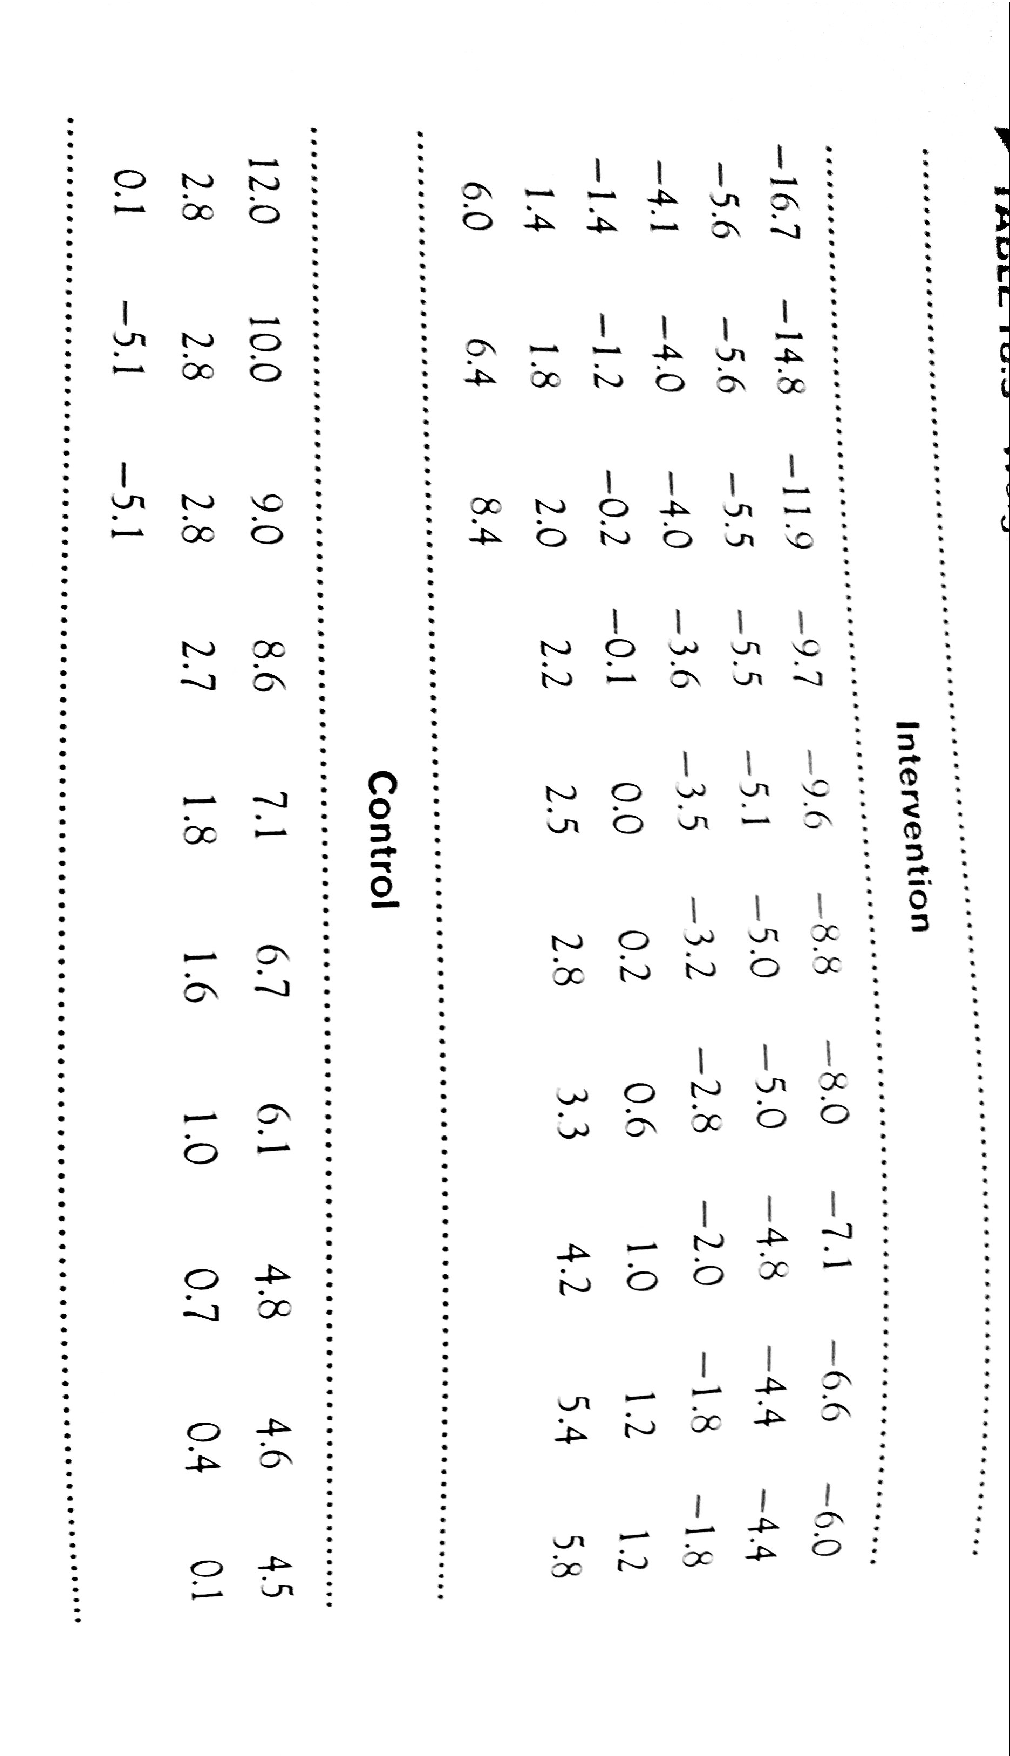
\includegraphics[scale=0.35, angle=90]{a83-crop.pdf} 
  \end{center}
  \caption{Weight change (lb) of obese children, by group}\label{fig:tab1}
\end{figure}

\clearpage

\section{Student drinking}\label{student-drinking}

A professor asked her sophomore students, ``How many drinks do you
typically have per session'' (A drink is defined as one 12-ounce beer,
one 4-ounce glass of wine, or one 1-ounce shot of liquor.) Some of the
students didn't drink. Table \ref{fig:tab2} gives the responses of the
female and male students who did drink. It is likely that some of the
students exaggerated a bit. The sample is all students in one large
sophomore-level class. The class is popular, so we are tentatively
willing to regard its members as an SRS of sophomore students at this
college.

\begin{enumerate}
\def\labelenumi{\alph{enumi}.}
\tightlist
\item
  Do a complete analysis that reports on a comparison of the drinking
  behavior of women and men.
\item
  Summarise your findings in a 140 character tweet.
\item
  (BONUS) Verify the constant variance assumption of your model.
\end{enumerate}

\begin{figure}[h]
  \begin{center}
    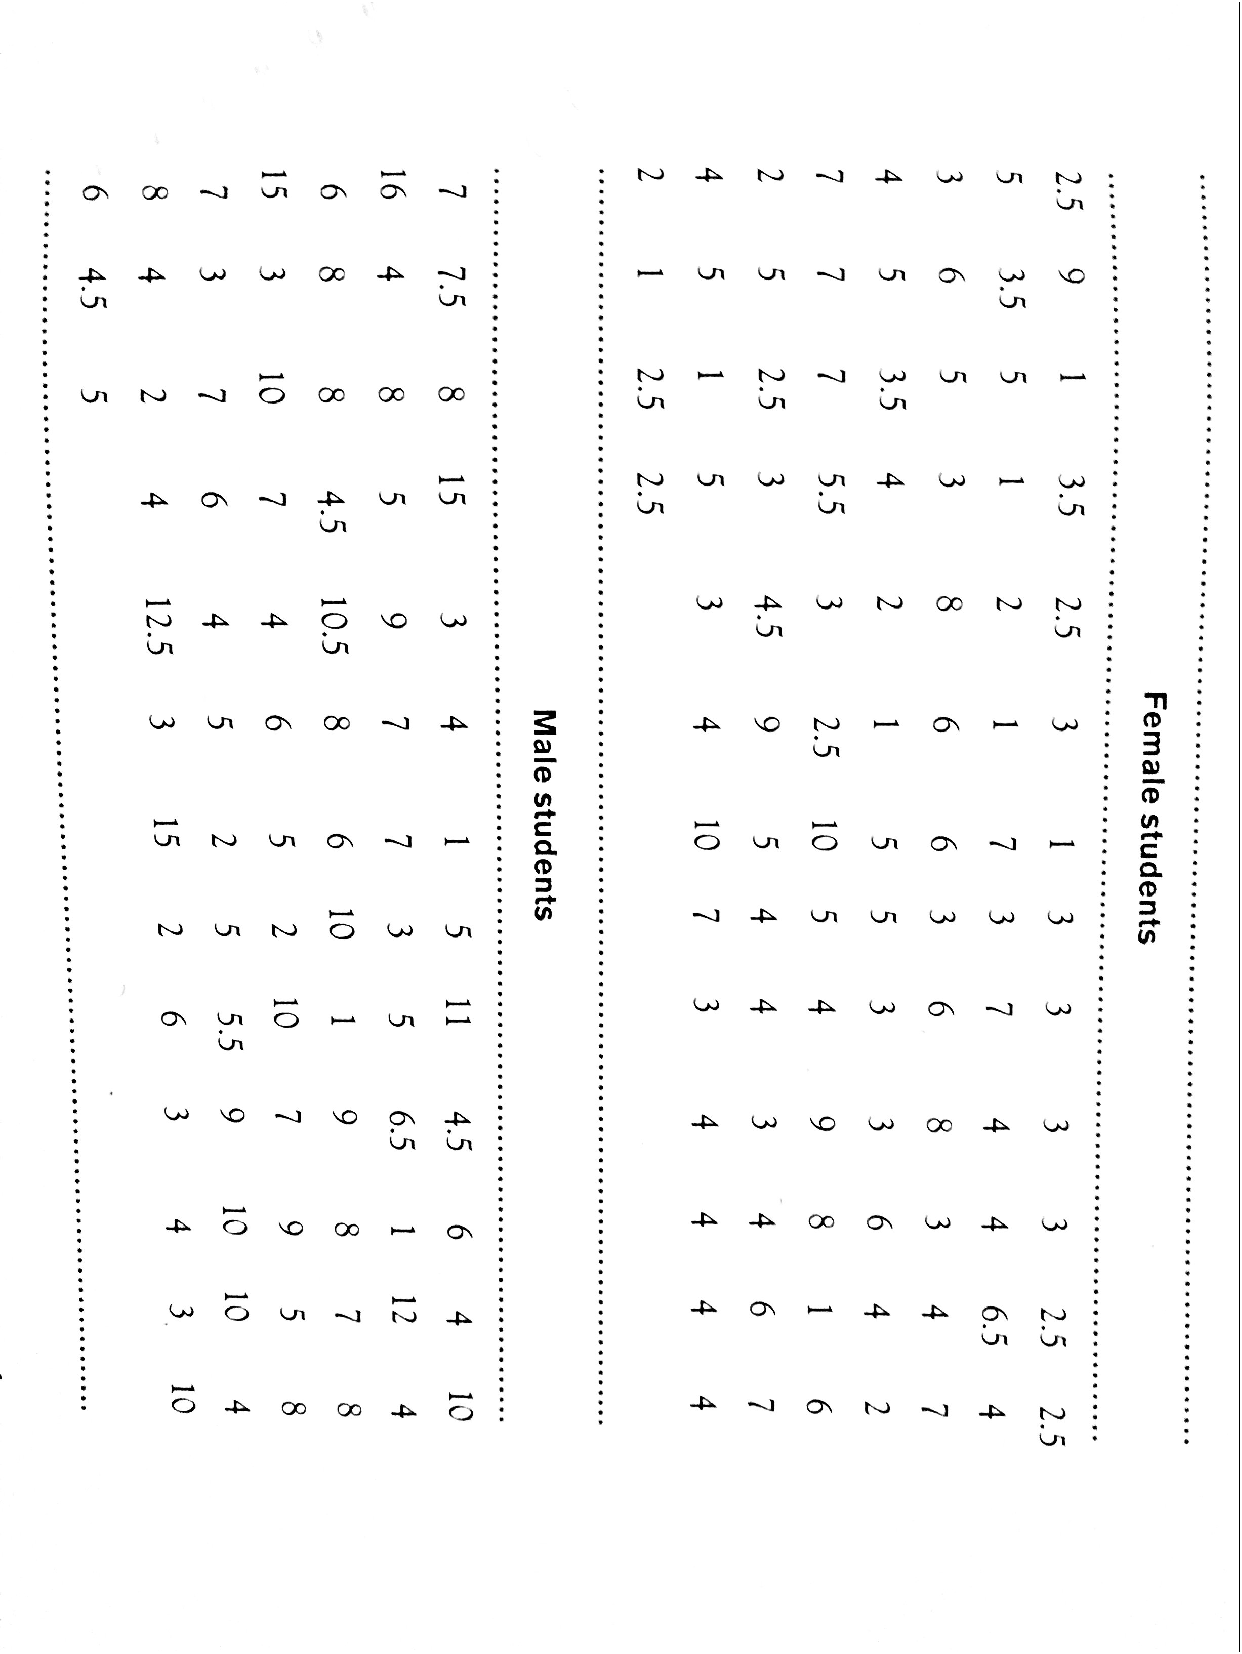
\includegraphics[scale=0.55, angle=90]{a81-crop.pdf} 
  \end{center}
  \caption{Drinks per session claimed by female and male students}\label{fig:tab2}
\end{figure}

\clearpage

\section{Ink toxicity}\label{ink-toxicity}

The National Toxicology Program evaluates the toxicity of chemicals
found in manufacturing, in consumer products, or in the environment
after disposal. Toxicity is assessed through a battery of tests. Here
are some results from a study of the toxicity of black newsprint ink in
7-week-old female rats. The rats' fur was locally clipped twice a week
for 13 weeks. One group of rats received a dermal application of ink
right after each clipping, and a control group of rats was left
untreated. Table \ref{fig:tab3} shows the body weights (in grams) of
female rats at the beginning of the study and at the end of the 13
weeks.

\begin{enumerate}
\def\labelenumi{\alph{enumi}.}
\tightlist
\item
  Verify that the two experimental groups are not significantly
  different at the beginning of the study
\item
  Is there good evidence that ink application impairs growth in female
  rats between 7 and 20 weeks of age? State your answer in terms of the
  \% difference between the mean weight gains of the two populations.
  Provide a 95\% confidence interval for the \% difference between the
  mean weight gains of the two populations.
\item
  Show how the p-value in the \texttt{glm} output was calculated for the
  parameter of interest.
\end{enumerate}

\begin{figure}[h]
  \begin{center}
    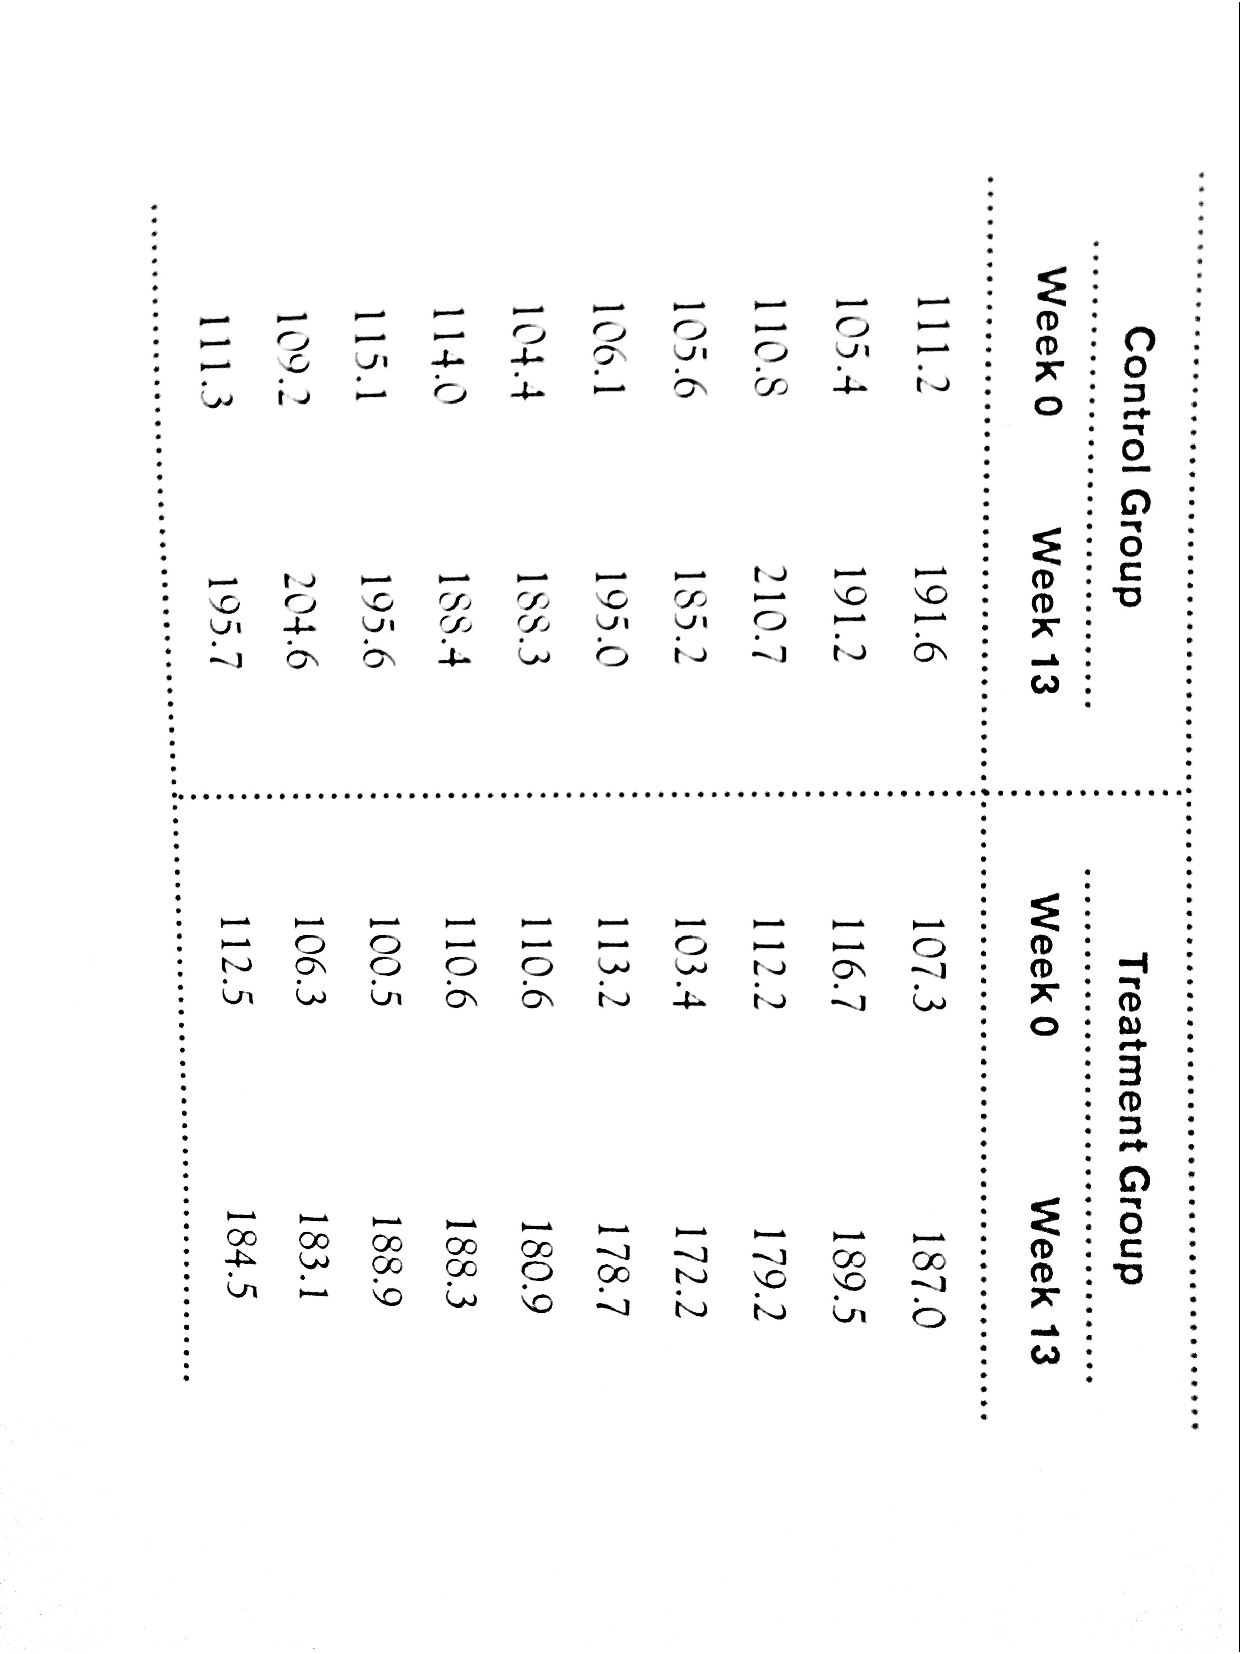
\includegraphics[scale=0.55, angle=90]{a82-crop.pdf} 
  \end{center}
  \caption{Body weights (g) at beginning and end of ink toxicity study}\label{fig:tab3}
\end{figure}

%\showmatmethods


\bibliography{pinp}
\bibliographystyle{jss}



\end{document}

